% put environments that should be ignored by texcount here, e.g., here listing for code

%TC:envir listing [] ignore

%for reference to this section
\section{Introduction}
\label{section:Introduction}
In today's world, nearly every industry uses 3D models to visually represent objects or environments. Whether for entertainment, development, or research, 3D models are essential tools for understanding complex concepts and ideas.
Another exemplary field is real estate development, where architects and engineers utilize Building Information Modeling (BIM). BIM improves collaboration and efficiency in construction projects by integrating various aspects of a building's lifecycle, from initial design through maintenance and deconstruction, into 3D models \autocite{azhar_building_2020}.


With modern interactive media, the demand for high-quality and numerous 3D models has significantly increased. Triple-A games and blockbuster movies heavily rely on detailed 3D models to create true-to-life experiences.

However, creating these models is a time-consuming and costly process that requires skilled artists and designers, especially when compared to capturing images or videos with cameras or smartphones. Recent advancements in Generative 3D AI have made it possible to generate 3D models from a single image, a process known as 3D object or mesh reconstruction.

While the generated models are currently not yet at the level required for Triple-A games or the high standards of the entertainment industry, it holds significant potential for transforming and partially automating the creation and use of 3D models. At present, these technologies are more suitable for smaller prototyping projects or indie productions.

Some examples of 3D mesh reconstruction include the newly released TripoSR (\textcite{tochilkin_triposr_2024}) as well as established models like Zero-1-to-3 (\textcite{liu_zero-1--3_2023}) and One-2-3-45 (\textcite{liu_one-2-3-45_2023}).

This paper provides an overview of the various approaches and models used for 3D mesh reconstruction, including a comparison of their performance, visual results and training based on 3D-model datasets such as Objaverse-XL \autocite{deitke_objaverse-xl_2023}.
It also explores the underlying methods and concepts like convolutional neural networks and neural radiance fields \autocite{mildenhall_nerf_2021} used in modern neural network-based models.
Finally, it offers a brief look at use cases and applications that benefit the most.
% \section{System Overview}
% Provide a high level overview of your system, approach, etc.
% Describe features, user interfaces, provide screenshots.
% What does a user do with your application/system/interaction method?

% \begin{listing}[H]
%     \begin{csharpcode}
%     for (var item in myList)
%     {
%         Console.WriteLine($"Fancy syntax highlighting for {item}");
%     }
%     \end{csharpcode}
%     \caption{Example of a listing.}
%     \label{lst:example}
% \end{listing}

% See code \ref{lst:example} for high efficiency code.

\section{Concepts and Functionality}
To understand the process of 3D mesh reconstruction, it is essential to explore the various techniques employed to generate 3D models from 2D images.

3D mesh reconstruction involves several methodologies, each contributing uniquely to the overall objective. Initial techniques like Shape from Shading \autocite{horn_shape_1989} utilized shading information to infer the 3D structure of objects. Multi-view Stereo (MVS) employed multiple images from different viewpoints to estimate 3D structure through triangulation methods.

The introduction of Convolutional Neural Networks (CNNs) significantly improved the accuracy of 3D reconstructions by providing robust tools for image analysis and feature extraction. Generative Adversarial Networks (GANs \autocite{goodfellow_generative_2014}) further enhanced these capabilities by providing a better training method.
Combining CNNs and GANs has led to advanced models such as Pixel2Mesh++ \autocite{wen_pixel2mesh_2019} and made it possible to accurately estimate a complete three-dimensional model from a single image.

Lastly Neural Implicit Functions, like NeRF \autocite{mildenhall_nerf_2021}, have further improved 3D reconstruction by using neural networks to model continuous volumetric functions which can generate high-quality 3D reconstructions with smooth surfaces.

The following sections examine each technique in detail, exploring their specific mechanisms, innovations, and contributions to the field.


\subsection{Shape from Shading}
Shape from Shading (SFS) is an early technique used to estimate the shape of an object from a single image, dating back to the late 80s (\textcite{horn_shape_1989}). This method aims to reconstruct the 3D shape of an object by analyzing shading information in a 2D image.

The idea of SFS is to use variations in shading to infer the 3D geometry of an object's surface. This method operates under several key assumptions:

\begin{enumerate}
    \item Lambertian Reflectance: The surface of the object reflects light uniformly in all directions. This means the intensity of reflected light depends only on the angle between the light source and the surface normal.
    \item Single Light Source: The object is illuminated by a single distant light source.
    \item Known Light Source Direction: The direction of the light source relative to the camera is known.
\end{enumerate}

When all assumptions are met, the intensity of the reflected light in relation to the incoming light direction can be used to estimate the surface normals at each point of the object. By integrating these normals, the depth of the object can be estimated, providing a 3D representation of the object.

While Shape from Shading is a robust technique, it has limitations. It requires accurate knowledge of the light source direction and assumes Lambertian reflectance, which does not hold up for real-world objects and results in a significant deviation from real light behavior \autocite{wolff_generalizing_1996}.
This problem is not just present in the SFS method but also in a lot of other computer graphics and computer vision appliances, as a compromise for computational efficiency and simplicity.
Additionally, the SFS is sensitive to noise and may produce inaccurate results in complex scenes.


\begin{figure}
    \centering
    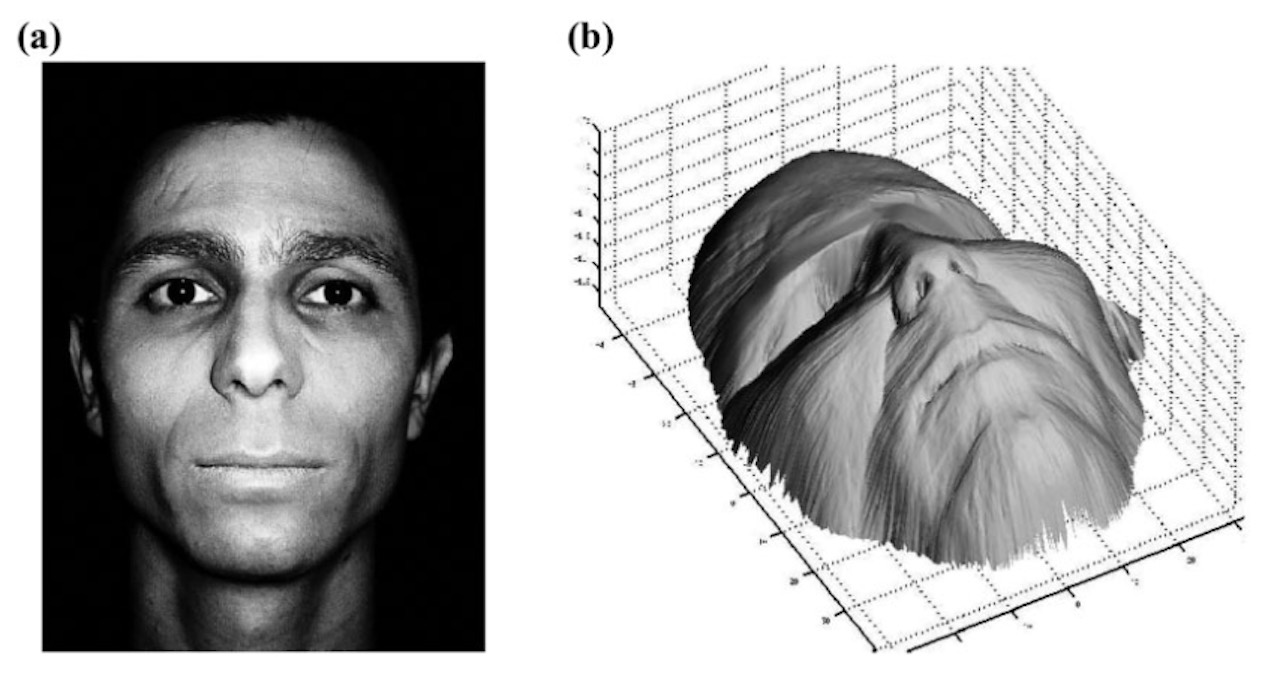
\includegraphics[width=0.9\linewidth]{images/shape_from_shading.jpg}
    \caption{(a) A real face image. (b) Surface recovered from (a) by the generic SFS algorithm with the perspective model, with the light source located at the optical center. (taken from \textcite{he_advances_2018})}
    \label{fig:shape_from_shading}
\end{figure}

\subsection{Multi-view Stereo}
Multi-view Stereo (MVS) uses multiple images of an object taken from different angles to estimate its 3D structure (see Figure \ref{fig:multi_view_stereo}). This concept, known as Structure from Motion (SfM), cannot be traced back to a single publication but is rather a collection of various works.
Ullman \autocite{ullman_interpretation_1997} was among the first to describe the process in a computational context, noting that the structure of four non-coplanar points can be recovered from three orthographic projections.

SfM involves the following steps:

\begin{enumerate}
    \item Camera Calibration: Estimating intrinsic and extrinsic camera parameters. This involves focal length, principal point as well as distortion of each camera.
    \item Feature Detection and Matching: Identifying and matching features using techniques like Difference of Gaussians (DoG) and Harris corner detection. \textcite{furukawa_accurate_2010} for example, proposed a robust and efficient algorithm based on these well-established techniques.
    \item Pose Estimation: Determining relative positions and orientations of cameras based on features.
    \item Triangulation: Using poses and features to estimate 3D points in the scene.
    \item Dense Reconstruction: Interpolating the sparse 3D points to create a solid 3D model.
\end{enumerate}

MVS has also gained significant relevance in augmented and virtual reality for real-time environment reconstruction and mapping.

Despite its effectiveness, MVS has limitations, such as requiring multiple images from different viewpoints, which may not always be available.
Moreover, MVS can struggle with textureless surfaces and repetitive patterns, which can make feature matching challenging.
These limitations have driven the development and adoption of deep learning methods, which can overcome some of these challenges by learning from large datasets of images and 3D models.

\begin{figure}
    \centering
    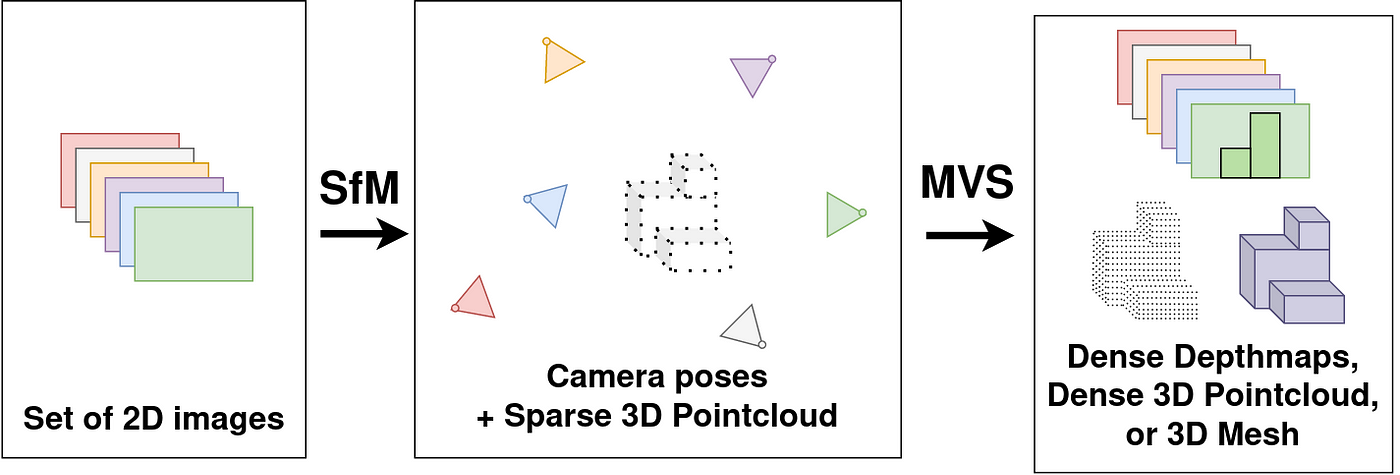
\includegraphics[width=1\linewidth]{images/multi_view_stereo.png}
    \caption{Multi-view Stereo Pipeline (taken from \textcite{rouch_patchmatch_2023})}
    \label{fig:multi_view_stereo}
\end{figure}

\subsection{Convolutional Neural Networks} \label{section:cnns}
Convolutional Neural Networks (CNNs) are deep learning models especially useful when working with image data. They have significantly impacted the field of computer vision and have found applications in many areas, including 3D mesh reconstruction.

CNNs usually operate on grid-like structures, processing data with convolutional layers that capture spatial hierarchies of features through a series of filters. This grid-based operation is particularly effective for image data, where the spatial arrangement of pixels is crucial for understanding the content.

Compared to traditional methods, like MVS, CNNs and the other following deep learning models can learn complex features from images and automatically extract relevant information for 3D reconstruction. They are also more robust to noise and variations in lighting conditions.
\paragraph{}
AlexNet by \textcite{krizhevsky_imagenet_2012} was one of the first successful applications of CNNs to image classification, achieving substantial performance improvements over previous methods. Specifically, AlexNet reduced top-1 error rates to 37.5\% and top-5 error rates to 17.0\%, which were significantly better than the previous state-of-the-art.
Top-1 and top-5 error rates are common metrics used to evaluate the performance of image classification models. The top-1 error rate is the percentage of images for which the correct label is not in the top-1 predicted labels, while the top-5 error rate is the percentage of images for which the correct label is not in the top-5 predicted labels.

\subsection{Generative Adversarial Networks} \label{section:gans}
Generative Adversarial Networks (GAN) \autocite{goodfellow_generative_2014} are a type of deep learning model that consists of two neural networks: a generator and a discriminator. The generator is responsible for generating new data samples, while the discriminator is responsible for distinguishing between real and generated data samples. The two networks are trained together in competition, where the generator tries to generate realistic data samples to fool the discriminator, and the discriminator tries to distinguish between real and generated data samples.
\paragraph{}
In the context of 3D mesh reconstruction, CNNs and GANs are often used together to generate 3D models from 2D images. The CNN is used to extract features from the input image, and the GAN is used to generate the 3D model from these features. One example of this is the Pixel2Mesh++ model by \textcite{wen_pixel2mesh_2019}.

\subsection{Neural Implicit Functions} \label{section:nif}
Neural Implicit Functions represent an alternative approach to 3D reconstruction by using neural networks to model continuous volumetric functions. Unlike traditional methods that use explicit representations like meshes or voxels, neural implicit functions encode the geometry of 3D objects in a continuous function that can be evaluated at any point in 3D space.

Neural Implicit Functions, such as DeepSDF \autocite{park_deepsdf_2019} and NeRF \autocite{mildenhall_nerf_2021}, use neural networks to map spatial coordinates to implicit representations of 3D shapes. These models learn a function that outputs a value indicating whether a point lies inside or outside the object (in the case of signed distance functions — DeepSDF) or the density and color at a given spatial location (in the case of radiance fields — NeRF).

\paragraph{}
Neural Implicit Functions usually work in the following steps:
\begin{enumerate}
    \item Data Collection: Collect dataset of 3D shaped and corresponding, annotated 2D images. An example of such a dataset is ShapeNet \autocite{chang_shapenet_2015}.
    \item Network Training: Training the network to minimize error between the predicted and actual shape representation using the loss function. This process is similar to the fooling of the discriminator in GANs (\ref{section:gans}).
    \item Shape Inference: Once trained, the network can infer the 3D shape from new inputs by querying the implicit function at various spatial locations to reconstruct the geometry.
\end{enumerate}

The main advantages of neural implicit functions include their continuous nature, which allows for high-quality reconstructions with smooth surfaces. Another advantage is the fact that they typically require less memory and computation compared to explicit representations like meshes or voxels created by deep convolutional networks like the aforementioned CNNs (\ref{section:cnns}).
NeRFs — Neural Radiance Fields \autocite{mildenhall_nerf_2021} have been particularly successful in generating high-quality 3D reconstructions from 2D images (see Figure \ref{fig:nerf}) and are used in almost all modern neural network-based 3D reconstruction models.


\begin{figure}
    \centering
    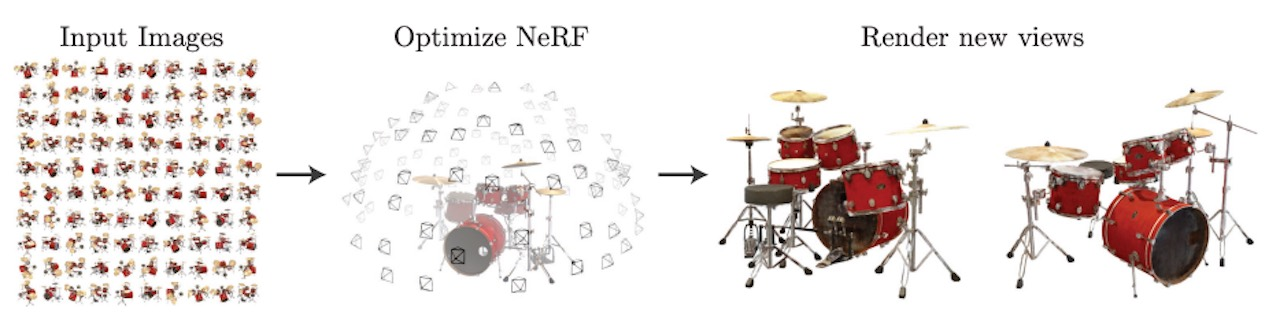
\includegraphics[width=1\linewidth]{images/nerf.jpg}
    \caption{NeRF - 100 input views to NeRF representation  \autocite{mildenhall_nerf_2021}}
    \label{fig:nerf}
\end{figure}

\section{Models}

In the recent years several models have been developed to generate 3D models from 2D images. Some of the most prominent models include:

\subsection{Pixel2Mesh}
Pixel2Mesh is a model developed by \textcite{wang_pixel2mesh_2018}.
It is built with two main components. The image feature network which is a convolutional neural network (CNN) that extracts perceptual features from the input image. The second component is a cascaded mesh deformation network which is a graph-based convolution network.

A graph-based convolution network differs from traditional CNNs in that it operates on a graph rather than a grid. In the context of Pixel2Mesh, the graph represents the 3D mesh model with vertices and edges.

\paragraph{}
The Pixel2Mesh model works in the following steps:
\begin{enumerate}
    \item The input image is passed through the image feature network to extract features.
    \item The cascaded mesh deformation network initializes with an ellipsoid mesh model.
    \item The features extracted from the image are then taken to refine the shape of the mesh model.
    \item The mesh model gets refined iteratively in 3 blocks, with each iteration refining the shape and increasing the mesh resolution. (see Figure \ref{fig:pixel2mesh})
    \item The vertex positions get estimated each step, which are then used to look up the features from the image feature network for the next iteration.
\end{enumerate}
\begin{figure}
    \centering
    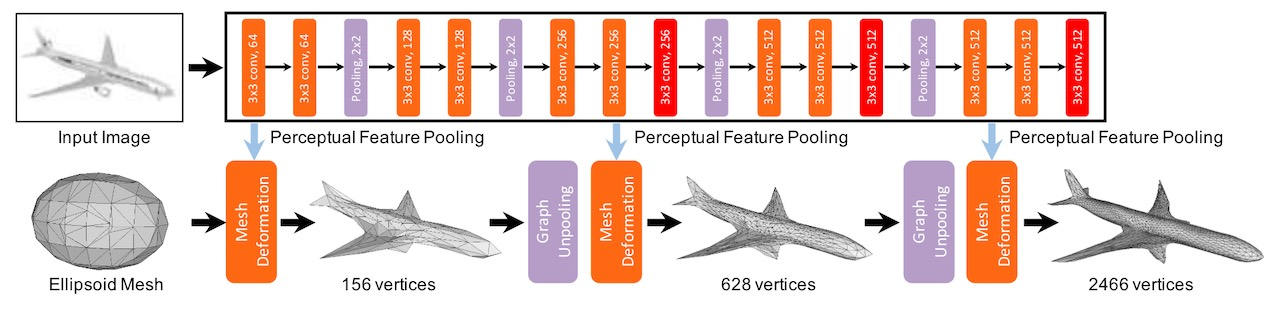
\includegraphics[width=1\linewidth]{images/pixel2mesh.jpg}
    \caption{Pixel2Mesh Pipeline \autocite{wang_pixel2mesh_2018}}
    \label{fig:pixel2mesh}
\end{figure}

\subsection{Pixel2Mesh++} \label{section:pixel2meshpp}
Pixel2Mesh++ \autocite{wen_pixel2mesh_2019} is an adaption of the original Pixel2Mesh model.  Instead of using a single image, it relies on multiple images to generate a more accurate 3D model.
It mixes the already well-known MVS systems with the Pixel2Mesh model.

Pixel2Mesh++ operates by sampling deformation around each vertex of the base mesh and selecting the optimal deformation using perceptual features pooled from multiple input images. This multi-view approach enables the model to capture more detailed and accurate geometries, especially in occluded or less visible areas, where single-view methods cannot capture the full extent of an object and need to estimate the shape by hallucinating the missing parts — hence this model is included in this overview.

\subsection{Zero-1-to-3} \label{section:zero123}
The Zero-1-to-3 (Zero123) model, developed by \textcite{liu_zero-1--3_2023}, is designed to generate 3D models from a single image in a zero-shot manner, meaning it can produce accurate 3D reconstructions without needing extensive per-object training. Compared to Pixel2Mesh, this model creates not just the mesh, but also a colored texture based on the given image. This model highlights its robustness and versatility across various types of input images.

The process involves fine-tuning a pre-trained diffusion model, in this case Stable Diffusion, to learn how to control camera extrinsics (the external parameters defining the camera's position and orientation).
By using a 3D model dataset, the model learns to manipulate the camera viewpoint. This allows it to create views from certain angles — also called novel view synthesis which can be observed in Figure \ref{fig:zero-1-to-3}.

By merging the input image with the synthesized views, the model can effectively learn the 3D structure of the object and generate a high-quality 3D mesh.

The retrained version, Zero123-XL, further improves the performance by including additional training data. Zero-1-to-3-XL makes use of the extensive dataset Objaverse-XL \autocite{deitke_objaverse-xl_2023}, which contains over 10 million 3D objects.
This larger dataset allows the model to enhance its zero-shot capabilities and overall reconstruction accuracy.

\begin{figure}
    \centering
    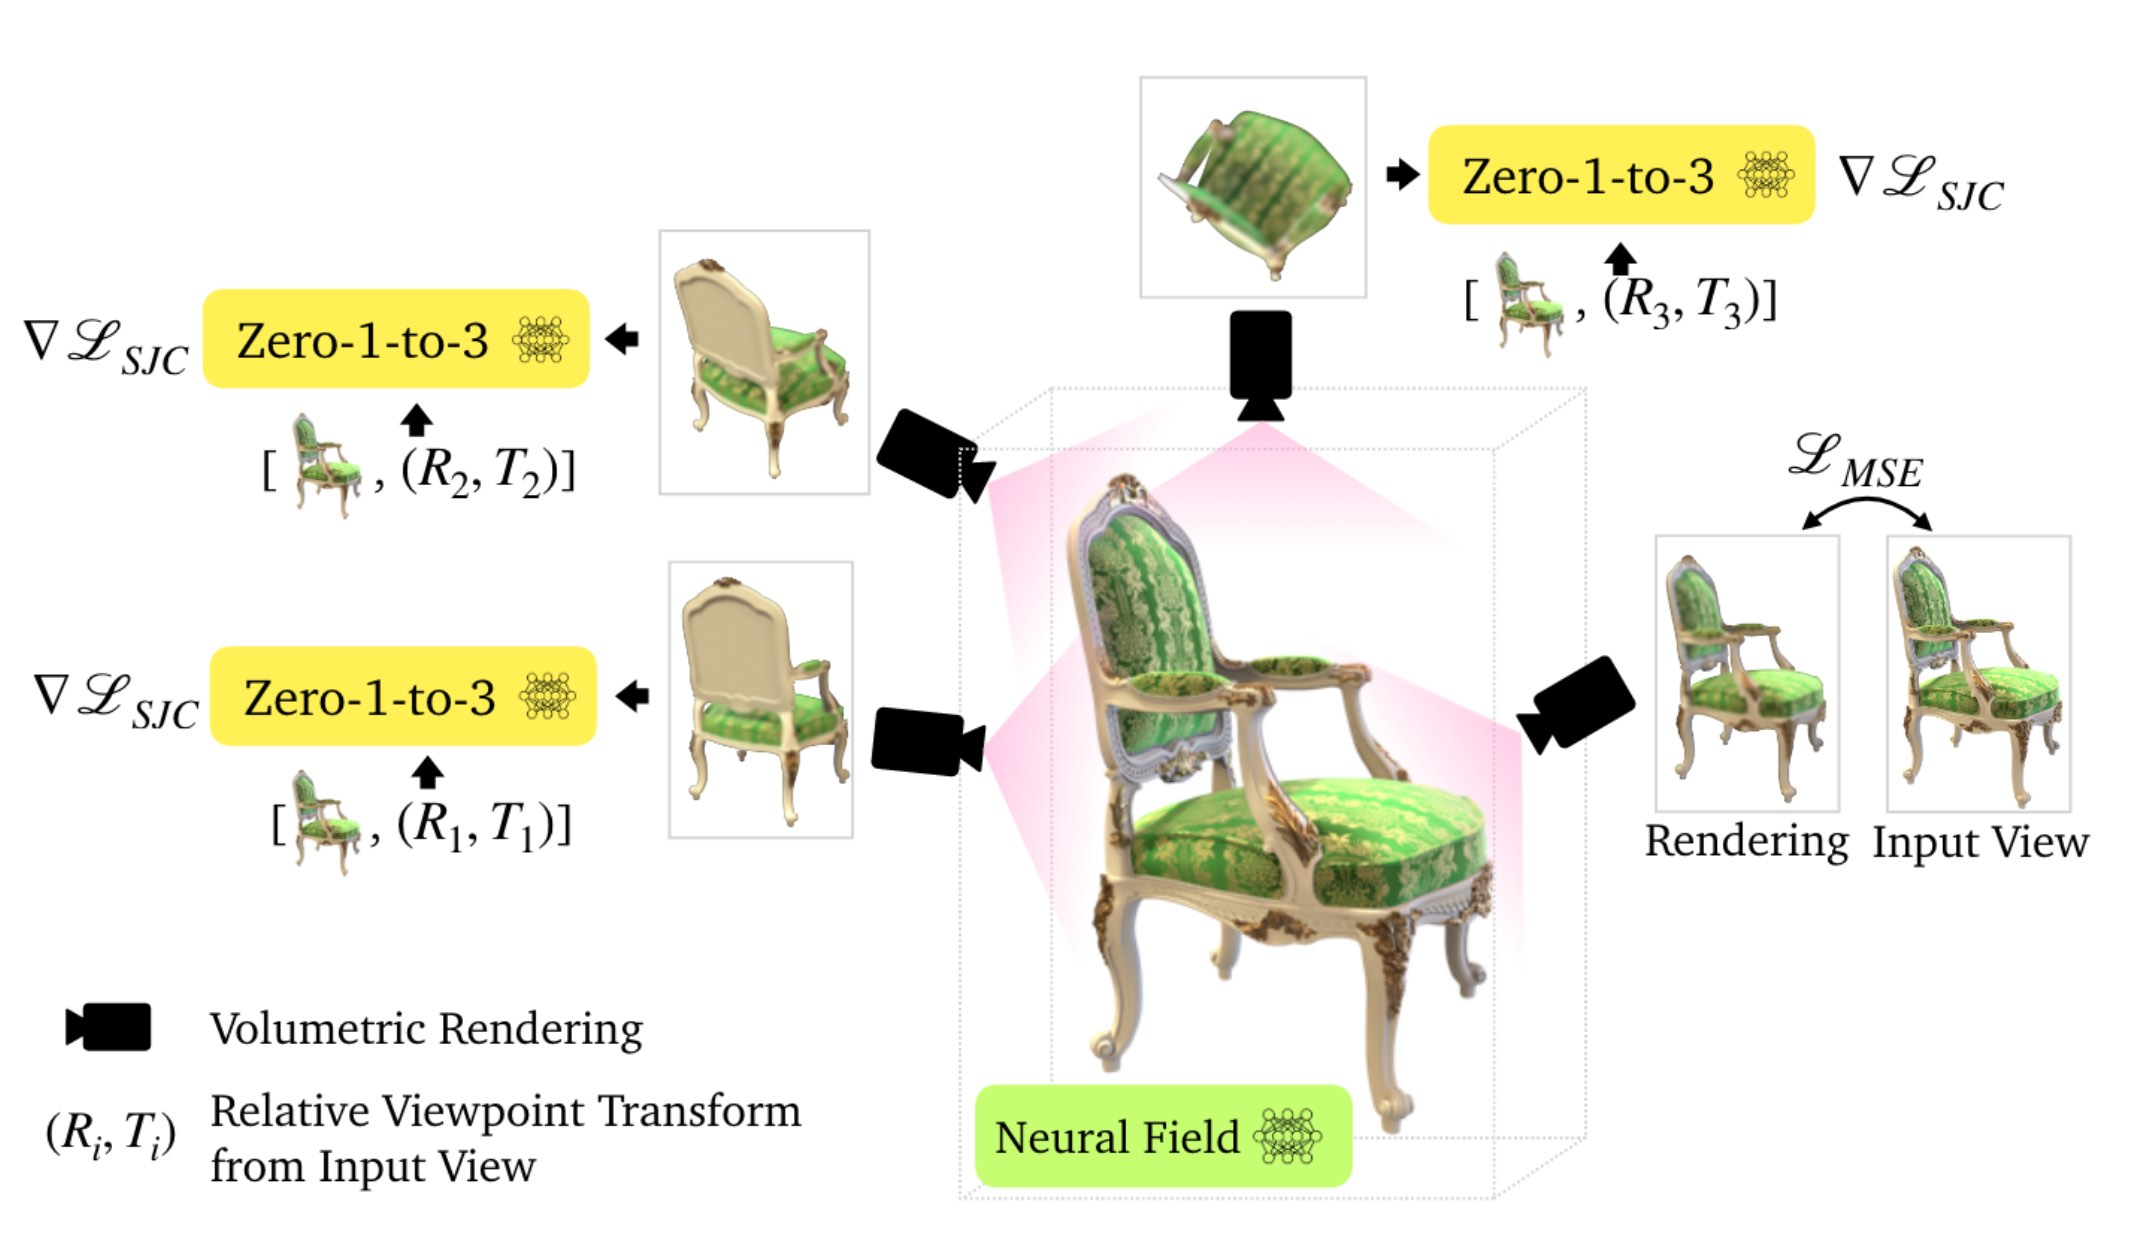
\includegraphics[width=0.9\linewidth]{images/zero-1-to-3.jpg}
    \caption{3D reconstruction with Zero-1-to-3 \autocite{liu_zero-1--3_2023}. The model receives the base image as well as the view parameters \(R\) (Rotation) and \(T\) (Transform) as input.}
    \label{fig:zero-1-to-3}
\end{figure}

\subsection{One-2-3-45} \label{section:one-2-3-45}
One-2-3-45, developed by \textcite{liu_one-2-3-45_2023}, is a state-of-the-art model designed to generate 3D meshes from single 2D images with exceptional efficiency.

It can reconstruct a full 360-degree 3D textured mesh in just 45 seconds, significantly faster than other models, which often require lengthy optimization processes. This rapid processing is achieved without the need for per-shape optimization, making it far more suitable for real-time consumer applications.
One-2-3-45 uses the aforementioned Zero123 (\ref{section:zero123}) model to generate multi-view images from the input image. These images are then compared to the input image for pose estimation. The results are poses for each of the generated views.
These results are lastly fed into a signed distance function based neural surface reconstruction model (similar to DeepSDF mentioned in \ref{section:nif}) which generated the finished 3D mesh.

An improved version, One-2-3-45++ \autocite{liu_one-2-3-45_2024}, was later released, which further optimized the model's performance.
The biggest improvement was the switch from Zero123 to a custom 2D diffusion model. Zero123 tried to predict each view individually, which resulted in inconsistencies. The new model uses a fine-tuned 2D diffusion model, which can attend all views simultaneously, resulting in more accurate results.

\begin{figure}
    \centering
    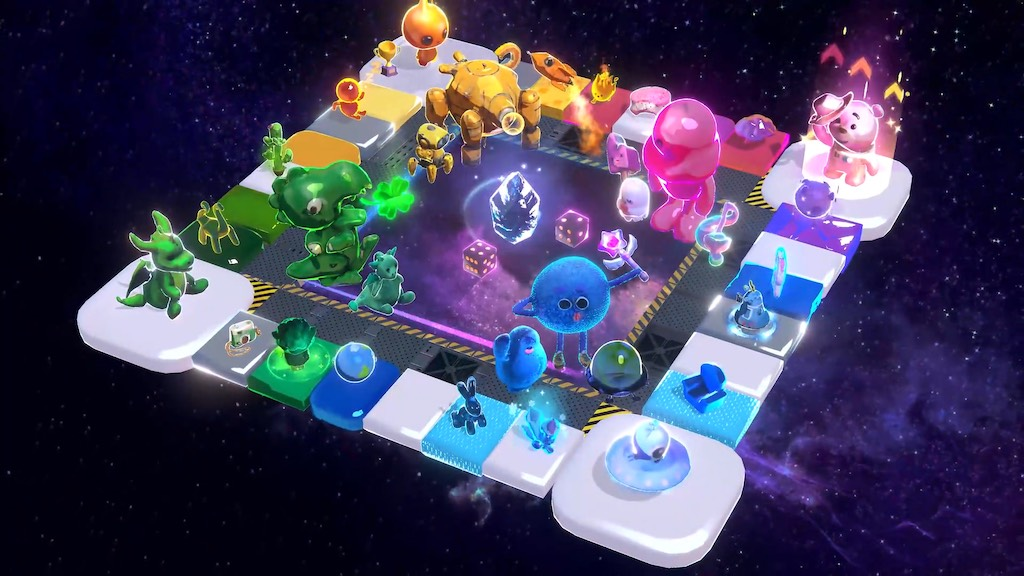
\includegraphics[width=1\linewidth]{images/one-2-3-45++_demo.jpg}
    \caption{Models generated by One-2-3-45++ \autocite{liu_one-2-3-45_2024}}
    \label{fig:one-2-3-4-5-plus-plus-demo}
\end{figure}

\subsection{TripoSR} \label{section:triposr}
TripoSR, developed by \textcite{tochilkin_triposr_2024}, is an another model for fast 3D object reconstruction from a single image.
It was created as a group effort by Stability AI (the creators of Stable Diffusion) as well as Tripo AI.
Building upon the Large Reconstruction Model (LRM) architecture by \textcite{hong_lrm_2024}, TripoSR uses transformer technology for feed-forward 3D generation, producing high-quality 3D meshes in under 0.5 seconds.

The LRM architecture consists of three main parts: an image encoder, a triplane representation, and a NeRF decoder. The image encoder, based on a vision transformer, takes an input image and converts it into a set of detailed features called latent vectors. These latent vectors capture important information about the object's shape and appearance in a compressed form.

Next, the triplane representation takes these latent vectors and arranges them in a three-dimensional grid. This grid captures the object's complex shapes and textures. The triplane representation uses layers that help the model focus on different parts of the image and learn how they relate to each other.

Finally, the NeRF decoder takes the 3D grid and predicts the color and density of each point in space, creating a smooth and detailed 3D model of the object.

TripoSR introduces several key improvements to this architecture. For example, it uses only a hand-selected higher quality subset of the Objaverse dataset, which improves generalization and reconstruction quality. It also introduces a mask loss function that penalizes differences between predicted and ground-truth mask images, reducing artifacts and improving reconstruction fidelity.

\subsection{Comparison}

\begin{figure*}
    \centering
    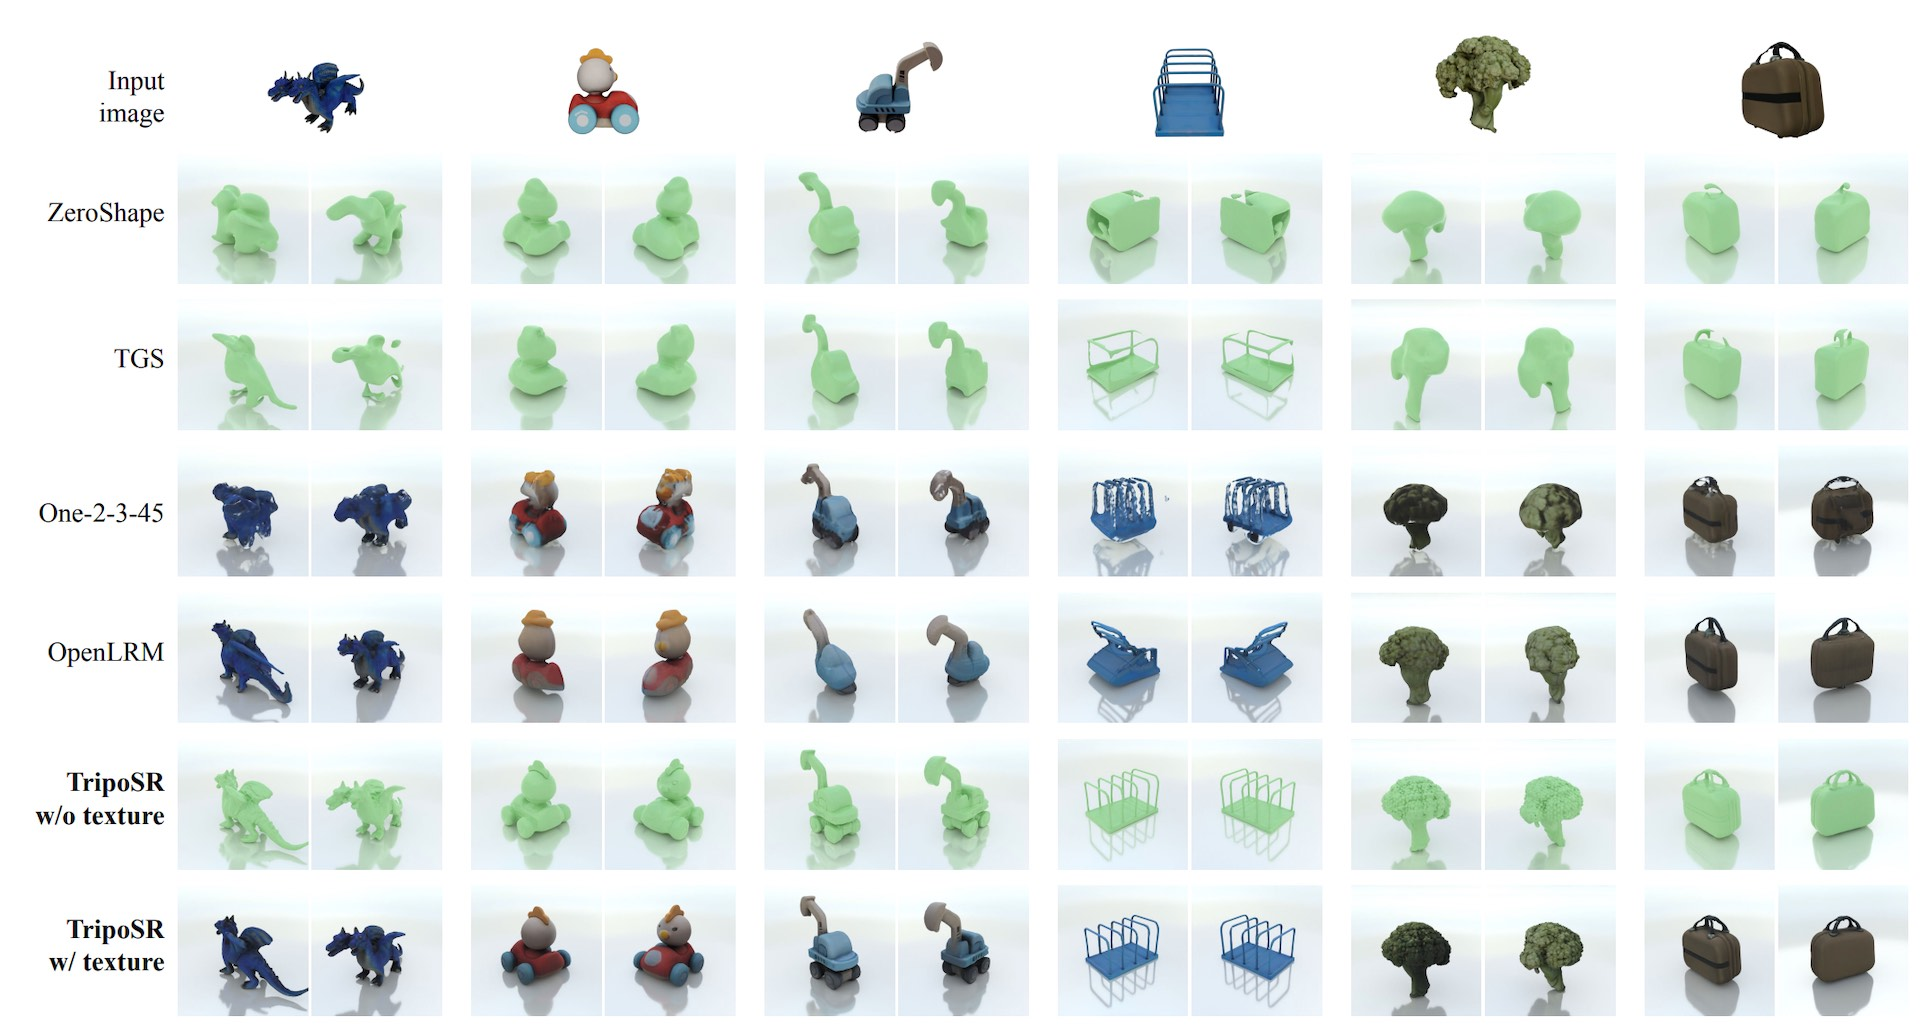
\includegraphics[width=0.8\textwidth]{images/comparison_tripo.jpg}
    \caption{Comparison of TripoSR to other state-of-the-art methods — including One-2-3-45 \autocite{tochilkin_triposr_2024}}
    \label{fig:comparison-tripo}
\end{figure*}

\subsubsection{Model Training}
Most models are trained on a 3D model dataset. A recent dataset, Objaverse-XL \autocite{deitke_objaverse-xl_2023} contains over 10 million 3D objects and is used by models like Zero123-XL to improve their zero-shot capabilities.
The term zero-shot in machine learning refers to the ability of a model to handle elements it has never seen before.
Just like with training Large Language Models, the 3D models in these datasets are crawled from various sources from across the internet.
This leads to ethical concerns regarding copyright and licensing.
In the case of Objaverse-XL, most models are sourced from open-source GitHub repositories but also some more specialized sites like Sketchfab, Thingiverse or Polycam.

\subsubsection{Model Performance}
Based on the order of the models listed above, each models reconstruction accuracy increases compared to the previous one.
Hence TripoSR (\ref{section:triposr}), the newest model, is the most accurate and efficient model.

Comparing models quantitatively can be done using metrics like Chamfer Distance (CD) and F-score (FS). The Chamfer Distance measures the average distance between points on the generated and ground-truth meshes, while the F-score, the harmonic mean of precision and recall, measures the overlap between the two meshes.

Compared to other models like One-2-3-45 (\ref{section:one-2-3-45}) and LRM, TripoSR is better in both speed and performance, as indicated by lower Chamfer Distance (CD \(\downarrow\)) and higher F-score (FS \(\uparrow\)) metrics on benchmark datasets. The scores of TripoSR are \(0.111\) and \(0.651\) respectively, while One-2-3-45 has scores of \(0.227\) and \(0.382\).
According to these values, TripoSR is about twice as accurate as One-2-3-45.

These metrics can also be visually proven by comparing the generated models side by side (see Figure \ref{fig:comparison-tripo}).

\subsubsection{Model Complexity}
Due to the lack of performance testing in this paper, all mentioned results are based on the respective papers.

As already mentioned, TripoSR (\ref{section:triposr}) is by far the fastest model, generating high-quality 3D models in under 0.5 seconds.
TripoSR is therefore about 10 times faster than LRM, the model it is based on, which takes about 5 seconds to generate a 3D object with less accuracy.
This is still significantly faster than for example One-2-3-45++ (\ref{section:one-2-3-45}), which takes about 60 seconds to generate a 3D object.

The other models compared did not provide exact time measurements.

All these measurements were taken using A100 GPUs, which are the state of the art in terms of AI performance with 80 GB of memory.

These graphics cards were also used in the training of these models. LRM was trained on 128 of these GPUs for 3 days.
A total of about 9000 hours at an energy consumption of 250 watts which results in 2.3 MWh. This might sound like a lot but when comparing to other AI models it's almost nothing.
The Large Language Model Llama \autocite{touvron_llama_2023} for example used 2048 of the A100 GPUs for 5 months, resulting in an about a thousand times higher energy usage of 1.8 GWh.

\section{Possible Applications}
As the field is still relatively new, no mainstream applications have been established yet. However, the potential is great, and some possible applications have already been identified.

\subsection{Development and Entertainment}
The most prominent application of 3D mesh reconstruction can be seen in the development and entertainment industry. The ability to generate 3D models from 2D images could revolutionize the asset creation process.
This would be especially beneficial for indie developers or small studios that do not have the resources to create high-quality 3D models from scratch. The generated models could be used in video games, movies, animations, and other forms of media. This significantly reduces the time and costs associated with creating 3D assets, allowing developers and animators to focus on other aspects of their projects. (see Figure \ref{fig:one-2-3-4-5-plus-plus-demo})

\subsection{Medical}
\begin{figure}
    \centering
    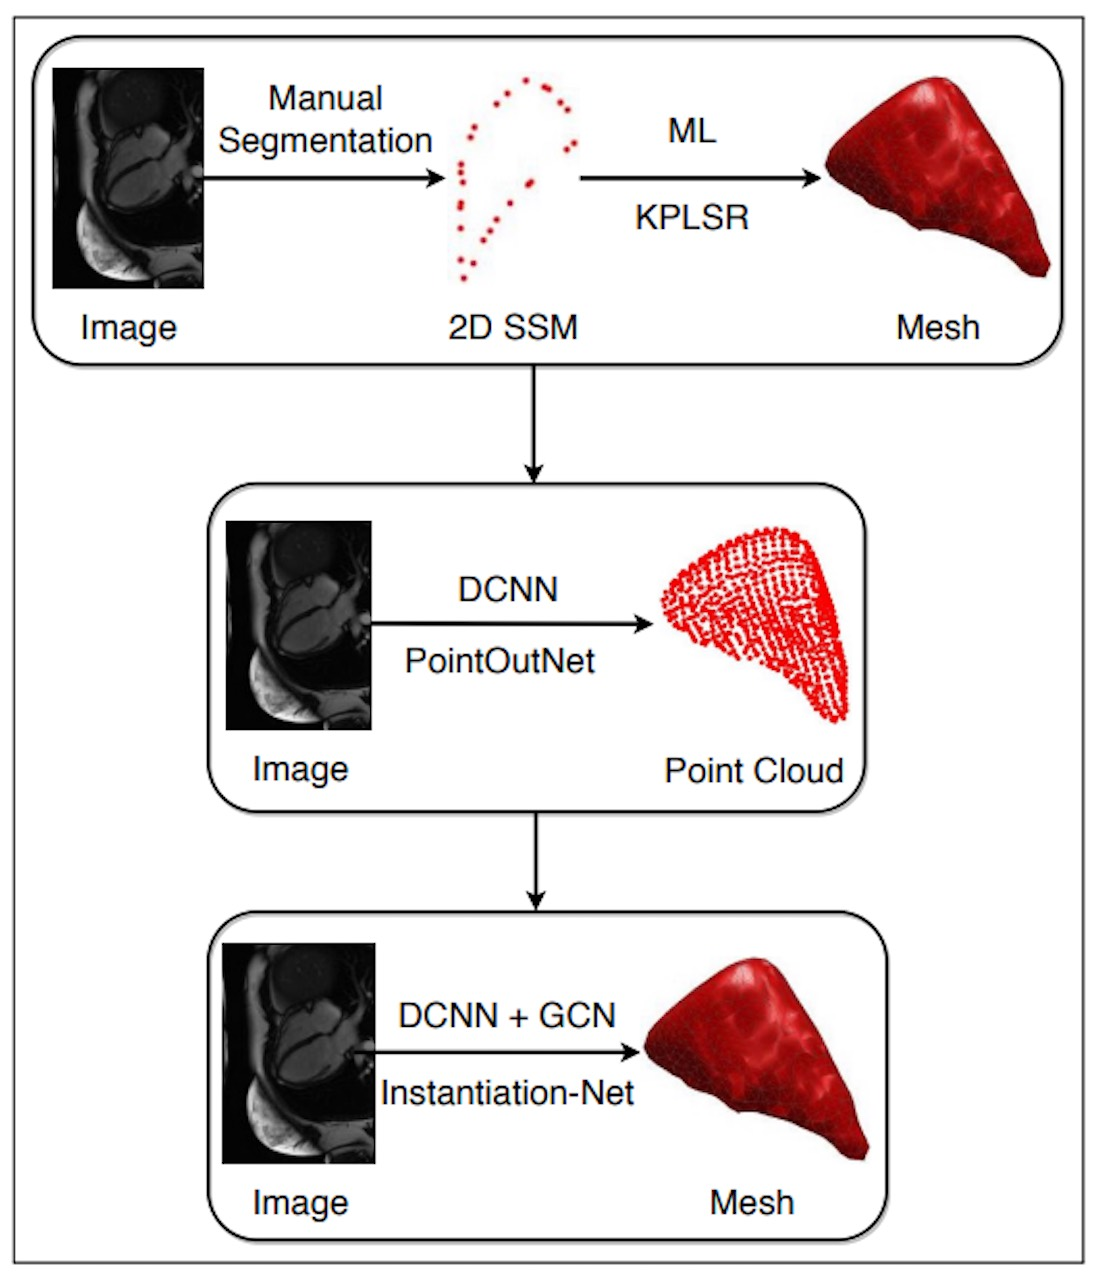
\includegraphics[width=0.7\linewidth]{images/medical.jpg}
    \caption{Medical Image Pipeline of Instantiation-Net \autocite{wang_instantiation-net_2019}.}
    \label{fig:medical}
\end{figure}

With Instantiation-Net, \textcite{wang_instantiation-net_2019} have shown that 3D mesh reconstruction can be used in the medical field to generate 3D models of organs from medical images. The whole pipeline can be seen in Figure \ref{fig:medical}. These models can be used for diagnosis, treatment planning, and medical education. For example, 3D models of the heart can be used to plan surgeries and visualize complex anatomical structures.

Diagnosing based on the 3D model also comes with risks and can potentially be problematic. The model is only an estimation based on training data and not a real representation of the patient's anatomy.

\subsection{Other Applications}
In the future 3D mesh reconstruction could also be used in fields like architecture, archaeology, cultural heritage, and many more.
There have just not yet been any significant uses of the technology in these fields. And it might also be necessary to adapt the models to the specific requirements of these fields.

% \section{Ethical Implications}
% Even though all the advancements in the field of 3D mesh reconstruction are promising, they also raise quite a few concerns.

% \subsection{Environmental Impact}
% Estimations of energy consumption for training as well as execution of models.

% \subsection{Training Data}
% The sources of training data. Looking at datasets like Objaverse-XL \autocite{deitke_objaverse-xl_2023} and their sources.

% \subsection{Privacy Concerns}

% \subsection{Cultural Sensitivity}
% It is important that the models are actually representative of the cultures, especially when generating models of people or culturally significant objects.

% \subsection{Implications of Estimations and Hallucinations}
% It is usually necessary for these models to estimate not seeable parts of the object. This can lead to hallucinations and other artifacts in the generated models.

% \section{Implementation}
% Provide implementation details such as the used software and our software architecture, highlight your own solutions to encountered difficulties. Describe relevant iterations of your implementation.

% Describe your methodology. How did you evaluate your work? Why did you choose this methodology? Present results of your evaluation here.

% Discuss your results to answer your research question. Does your data support you hypotheses? Put your results into perspective by situating it in the research field/related work.

\section{Conclusion and Future Direction}
Of all the models discussed, the most recent TripoSR model is the best in terms of accuracy and efficiency in almost any scenario.

Even though models are generating quite accurate 3D models, when given the right input images there is still room for improvement, especially with real world objects.

One aspect none of the mentioned models can handle are images with background. So at the moment, another model or manual intervention is necessary to remove the background from the image.

All mentioned models also assume Lambertian surfaces for the sake of simplicity, so the resulting models do not reconstruct shiny or metallic surfaces accurately.

The biggest roadblock of this technology is still clearly the fact, that there is just no way to see the backside of an object from the single taken image. Hence the estimated areas sometimes appear inaccurate or blurry.

% Summarize your work, outline limitations and future work.

% \section{Formatierung}
% \label{section:Formatting}

% Text mit beliebigen Sonderzeichen in UTF-8 ohne BOM \ldots
% ,
% \textbf{hervorgehobener Text},
% \texttt{void}\footnote{Fußnote 1},
% mathematische Formel im Text $\sum_{i=0}^n i^2$
% \ldots

% Referenz auf Unterabschnitt \ref{subsection:Coding} der Arbeit, automatisch richtig nummeriert.

% \textcite[]{Mulloni:2010} für einen einen Literaturverweis im laufenden Text.

% Literaturverweise sind essentiell für eine wissenschafliche Arbeit. \autocite[]{McConnell:2004:CCS:1096143}.

% Achtung: nur zitierte Literatur wird im Literaturverzeichnis
% angeführt.\footnote{Fußnote 2}


% Wir verwenden \LaTeX\footnote{ \url{http://en.wikibooks.org/wiki/LaTeX}} -- und das
% ist keine Quelle, sondern blos eine URL.

% \subsection{Figures machen was sie wollen}

% % h = try to place the figure Here
% % t = try to place the figure at the Top of a page
% % p = try to place this figure along with others on a separate Page
% % Note that LaTeX has a sophisticated ranking algorithm to place figures.
% % It is not always easy to accept LaTeX's placing but it is harder doing it
% % manually. Just let it go ;-)
% \begin{figure}[!ht]
% 	\centering
% 	\subfloat[Das Julia Fraktal]{
% 		\includegraphics[width=0.75\linewidth]{images/Julia-Fractal.png}
% 		%for reference of this subfigure only
% 		\label{subfigure:Julia-Fractal}
% 	}
% 	\qquad
% 	\subfloat[Noise für Tinteneffekte]{
% 		\includegraphics[width=0.75\linewidth]{images/Perlin-Coherent.png}
% 		%for reference of this subfigure only
% 		\label{subfigure:Perlin-Coherent}
% 	}
% 	\caption[
% 		Verschiedene Pixelgraphiken\newline
% 		% source url given in the table of figures
% 		\small\texttt{https://mediacube.at/wiki/}
% 	]{
% 		Verschiedene Pixelgraphiken
% 	}
% 	%for reference to all subfigures
% 	\label{figure:PixelImages}
% \end{figure}

% Unterstützte Pixelgraphikformate: PNG, JPEG, PDF.
% Angabe von height oder width meist wichtig.

% Referenz auf Abbildung \ref{figure:PixelImages} mit allen Teilbildern.
% Referenz auf Unterabbildung \ref{subfigure:Julia-Fractal}.

% %figure* stretches figure over both columns
% \begin{figure*}[t]
% 	\centering
% 	\includegraphics[width=0.9\textwidth]{images/KappaGamma.pdf}
% 	\caption{
% 		Vektorgraphik mit \LaTeX\ Beschriftung ($\kappa$, $\gamma$)
% 	}
% 	%for reference to this figure
% 	\label{figure:KappaGammaTau}
% \end{figure*}

% Referenz auf Abbildung \ref{figure:KappaGammaTau}.

% Bei Vektorgraphik mit \LaTeX\ Beschriftung keine Skalierung mit width oder height verwenden.

% Vektorgraphik mit \LaTeX\ Beschriftung kann etwa mit \texttt{ipe} erstellt werden.

% Unterstütztes Vektorgraphikformat: PDF. EPS muss konvertiert werden.


% \subsection{Unterabschnitt 2}
% %for references to this subsection
% \label{subsection:Coding}

% \begin{listing}[H]
%     \begin{csharpcode*}{firstnumber=10}
%         while (true)
%         {
%             // Ignition
%         }
%     \end{csharpcode*}

%     \caption{Example of another listing.}
%     \label{lst:Main}
% \end{listing}

% Wie man in Listing \ref{lst:Main}, kann man die erste Zeilennummern im Listing absichtlich ändern, hier z.B. auf 10. Beachte, dass man hier chsarpcode* als Umgebung nutzt, um neben
% den Default-Settings zusätzliche Einstellungen zu tätigen.

% \subsubsection{Unterunterabschnitt i}

% Wörtliches Zitat:
% %select proper language if not in German
% \selectlanguage{english}
% \begin{quote}
% ``Erwin Unruh discovered that templates can be used to compute
% something at compile time. [...] The intriguing part of this exercise, however, was that the production of the prime numbers was performed by the compiler during the compilation process and not at run time.''

% \autocite[305]{Bosch2014}
% \end{quote}
% %select German again or the language that you were using before (note ngerman stands for New German)
% %\selectlanguage{ngerman}
% \selectthesislanguage


% \subsection{Unterabschnitt b}

% \begin{enumerate}
% 	\item Punkt 1
% 	\begin{enumerate}
% 		\item Unterpunkt 1
% 		\item Unterpunkt 2
% 	\end{enumerate}
% 	\item Punkt 2
% \end{enumerate}

% \begin{itemize}
% 	\item Punkt 1
% 	\begin{itemize}
% 		\item Unterpunkt 1
% 		\item Unterpunkt 2
% 	\end{itemize}
% 	\item Punkt 2
% \end{itemize}


% \subsection{Unterabschnitt c}

% \begin{table}[ht]
% 	\centering
% 	\begin{tabular}{r|rrr}
% 		    & $i$ & $j$ & $k$ \\ \hline
% 		$i$ &$-1$ & $k$ &$-j$ \\
% 		$j$ &$-k$ &$-1$ & $i$ \\
% 		$k$ & $j$ &$-i$ &$-1$
% 	\end{tabular}
% 	\caption{
% 		Multiplikationstabelle für Quaternionen
% 	}
% 	\label{table:Quaternions}
% \end{table}

% Referenz auf Tabelle \ref{table:Quaternions}.

% \section{Abschnitt 2}
% \label{section:MathematicalStuff}

% Sei $f(x)$ eine stetige Funktion, so ist die \textbf{Fourier Transformierte}
% $F(\omega)$ wie folgt definiert:
% \begin{equation}
% \label{equation:FourierDefinition}
% 	F(\omega) = \int_{-\infty}^{\infty} f(x) e^{-i\omega t} dt
% \end{equation}

% Referenz auf mathematische Gleichung (\ref{equation:FourierDefinition}).

% Unnummerierte Gleichung:
% \begin{equation*}
% 	e^{i\varphi} = \cos\varphi + i \sin\varphi
% \end{equation*}
% %you may also use \[ \] instead of \begin{equation*} and \end{equation*}

% Gleichungssystem:
% \begin{eqnarray}
% 	g(x) = f(x - x_0) & \Leftrightarrow &
% 		G(\omega) = F(\omega) e^{-i\omega x_0} \\
% 	g(x) = f(x) e^{i\omega_0 x} & \Leftrightarrow &
% 		G(\omega) = F(\omega - \omega_0)
% \end{eqnarray}
